\documentclass[../main.tex]{subfiles}

\begin{document}
\chapter{The Website — Designing and Implementing an Elegant Interface} \label{ch:website}
    There were two options for how to implement the user interface: a desktop
        application or a website.
    A desktop application would have allowed users to run their programs locally,
        meaning they could safely use any Haskell library they wanted.
    However, this would have required users to download and install both the
        application, and Haskell itself, which could alienate users who are not
        familiar or comfortable installing software.
    A website, on the other hand, would allow users to run their programs in the
        browser, without needing to install anything.
    This would make the system more accessible to users, as they could use it on
        any device with a web browser.
    Additionally, a website would allow users to easily share their programs with
        others, by simply sending them a link to the website.
    For these reasons, it was decided to implement the system as a website.

    This website is the main interface for the user to interact with the system,
        and as such, it is important that the website is user-friendly and easy to use.
    This chapter will discuss its design and implementation, as well as the
        technologies used to build it.

    \section{Design Principles}
        Websites have been at the core of people's lives for the past two decades.
        They are used for a wide variety of activities, from shopping, to socializing,
            to filing taxes.
        It is therefore essential that websites meet certain design standards, to
            ensure that users can easily navigate them and find the information they need.
        It is also important that websites are visually appealing, to keep users
            engaged.
        As a result of these requirements, many standard website design practices have
            emerged over the years, which are important to consider when designing a
            website.

        \subsection{Purpose — What is the website for and what do we need to achieve that?}
            The first thing to consider when designing a website is its purpose.
            What is the website for?
            What is the user trying to achieve by visiting the website?
            These are important questions to ask, as they will help guide the design
                process.
            In the case of this project, the website is designed to allow users to write
                and run programs in Haskell, integrating seamlessly with the graphics library
                discusses in Chapter~\ref{ch:graphics}, and to view the results of their
                programs in both textual and graphical form.

            It would be easy to say that a Haskell editor, integrated with the graphics
                library would be sufficient for the website, and to ignore any further
                functionality.
            However, this would be a mistake.
            The website should be designed to be as user-friendly as possible, and to
                provide users with all the tools and information they need to achieve their
                goals.
            This means that alongside the Haskell editor, the website should feature a
                reference page where users can learn about the graphics library and how to use
                it, as well as an engaging homepage that showcases the capabilities of the
                library and encourages users to try it out.
            It would also be useful to allow users to save their programs and share them
                with others.

            These requirements lend themselves to a website with four main pages:
            \begin{itemize}
                \item A homepage, showcasing the capabilities of the graphics library and
                      encouraging users to try it out.
                \item A Haskell editor, integrated with the graphics library, where users can
                      write and run programs.
                \item A reference page, where users can learn about the graphics library
                      and how to use it.
                \item An account page, where users can view and manage their saved programs.
            \end{itemize}

        \subsection{Key Considerations}
            \subsubsection{User Experience — How can we make the website easy to use?}
                User experience is a key consideration when designing a website.
                The website should be easy to use, with a clear and intuitive interface that
                    guides users through the various features and functions of the site.
                Most websites follow a standard layout, with a header at the top of the page
                    containing the site's logo and navigation links, a main content area in the
                    centre of the page, and a footer at the bottom of the page containing
                    additional links and information.
                It is also generally recommended limiting text to no more than 80 characters
                    wide, as longer or shorter lines can make it difficult for users to read the
                    text.
                This layout, shown in Figure~\ref{fig:webLayout}, is familiar to users and
                    helps them navigate the site more easily.

                \begin{figure}[H]
                    \centering
                    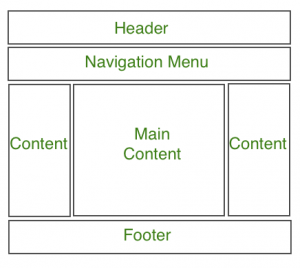
\includegraphics[width=0.45\linewidth]{images/webLayout.png}
                        \caption{Standard website layout.
                            Image taken from \href{https://www.geeksforgeeks.org/css-website-layout/}{Geek
                                    for Geeks: CSS Website Layout}.
                        }
                        \label{fig:webLayout}
                \end{figure}

            \subsubsection{Visual Design — How can we make the website visually appealing?}
                Visual design is another important consideration when designing a website.
                The website should be visually appealing, with a clean and modern design that
                    reflects the brand and purpose of the site.
                The website should use a consistent colour scheme and typography, with clear
                    and legible text.
                Images and graphics can also be used to enhance the visual appeal of the site,
                    but should be used sparingly and in a way that complements the overall design.

                \begin{figure}[H]
                    \centering
                    
\includegraphics[width=0.45\linewidth]{images/haskell.png}
                    
\includegraphics[width=0.45\linewidth]{images/haskellGrey.png}
                        \caption{Coloured Haskell logo (left) and monochrome Haskell logo (right).
                            Images taken from \href{https://www.haskell.org/}{Haskell.org} and
                                \href{https://wiki.haskell.org/Haskell_logos}{Haskell Wiki}.
                        }
                        \label{fig:haskell}
                \end{figure}

                For this website, it makes sense to use a colour scheme which reflects the use
                    of Haskell as the programming language.
                The website's colour scheme is based on the Haskell logo, shown in
                    Figure~\ref{fig:haskell}.

            \subsubsection{Accessibility — How can we make the website accessible to all users?}
                Accessibility is an important consideration when designing a website.
                The website should be accessible to all users, including those with
                    disabilities.
                This means that the website should be designed with accessibility in mind, with
                    features such as alt text for images, keyboard navigation, and high contrast
                    text.
                The website should also be compatible with screen readers and other assistive
                    technologies, to ensure that all users can access the content of the site.
                The website should also be responsive, meaning that it should adapt to
                    different screen sizes and devices.

    \section{Implementation}
        \subsection{Technologies}
            There are a number of technologies at play in the implementation of the
                website.
            While all websites are built on some combination of HTML, CSS, and JavaScript,
                there are a number of frameworks, libraries and tools that can be used to make
                the development process easier and more efficient.

            \subsubsection{TypeScript}
                The first of these is TypeScript, a superset of JavaScript that adds static
                    typing to the language.
                TypeScript compiles down to plain JavaScript, so it can be run in any web
                    browser, but the addition of static typing makes it easier to catch errors at
                    compile-time, rather than at runtime.
                This can help to prevent bugs and make the codebase more maintainable, as well
                    as saving a large amount of time in debugging.

            \subsubsection{React}
                React is a JavaScript library for building user interfaces.
                It is maintained by Facebook and is widely used in the industry.
                React allows developers to build reusable components that can be used to create
                    complex user interfaces.
                React components are written in JSX, a syntax extension for JavaScript that
                    allows developers to write HTML-like code directly in their JavaScript files.
                Similarly to TypeScript, React compiles down to plain JavaScript, HTML, and
                    CSS, so it can be run in any web browser.

                React provides full support for building single-page applications, which load a
                    single HTML document and then dynamically update the content of the page using
                    JavaScript.
                This can help to improve the performance of the website, as it reduces the
                    number of requests that need to be made to the server, as well as providing a
                    smoother user experience.

            \subsubsection{Next.js}
                Next.js is a framework built on top of React.
                It is one of the most popular frameworks for building websites, and the
                    decision to use it here was based largely on familiarity with the framework.
                Next.js provides numerous built-in optimizations for performance and SEO, and
                    makes it very easy to communicate between the client and server.
                It also provides a number of tools for handling routing, data fetching, and
                    other common tasks in web development.

                As with React, Next.js fully supports single-page applications.
                Next.js uses a file system-based routing system, where each page of the website
                    is represented by a file in the project directory.
                This makes it easy to add new pages to the website, as developers only need to
                    create a new file in the correct location.

            \subsubsection{Material UI}
                There are a number of user interface libraries available, which provide a set
                    of pre-built components that can be used to build websites.
                One of the most popular of these is Material UI, a library of highly
                    customisable React components that implement Google's Material Design
                    guidelines.
                Using Material UI can save time in development, as developers do not need to
                    spend time building components from scratch.
                Material UI also provides a consistent look and feel across the website, which
                    can help to improve the user experience.

            \subsubsection{MongoDB}
                MongoDB is a NoSQL database that stores data in a flexible, JSON-like format.
                It is widely used in the industry for its scalability and flexibility, as well
                    as its ease of use.
                Any database could have been used for this project, but as with Next.js,
                    MongoDB was chosen for its ease of use and familiarity.

        \subsection{File Structure}
            As mentioned earlier, the website is designed to have four main pages: a
                homepage, a Haskell editor, a reference page, and an account page.
            In reality, there are a few additional pages, such as a login page, a
                registration page, and a privacy policy page.
            The website uses Next.js App Router to handle routing between pages.
            As a file-system based router, Next.js uses the file structure of the project
                directory to determine the routes of the website.
            Each page of the website is represented by a file in the \texttt{app} directory
                of the project.
            For example, the homepage of the website is represented by the file
                \texttt{app/page.tsx}, the Haskell editor is represented by the file
                \texttt{app/editor/page.tsx}, and so on.

            The full structure of the website is as follows:
            \begin{itemize}
                \item \texttt{public/} — Contains all the static files used by the website, such as
                      favicon, and in this case, the source code for the graphics library.
                \item \texttt{src/} — Contains all the code to build the website.
                      \begin{itemize}
                          \item \texttt{actions/} — Contains all Next.js server actions.
                                These are functions that are called on the server side when a request is made
                                    to the website.
                          \item \texttt{app/} — Contains the pages of the website.
                                Next.js uses this directory to determine the routes of the website.
                          \item \texttt{assets/} — Contains all assets used by the website, such as images.
                          \item \texttt{components/} — Contains all React components used to build each page of
                                the website.
                          \item \texttt{contexts/} — Contains all React context providers used to manage the state
                                of the website.
                                Contexts provide a way to pass data through the component tree without having
                                    to pass props down manually at every level.
                          \item \texttt{database/} — Contains all the code to interact with the database.
                          \item \texttt{hooks/} — Contains all custom React hooks used by the website.
                                These are special functions that allow developers to "hook into" certain React
                                    features.
                          \item \texttt{schemas/} — Contains all the schemas used to validate the data sent to and
                                received from the server.
                          \item \texttt{styles/} — Contains all the CSS files used to style the website.
                          \item \texttt{middleware.ts} — Contains the logic to handle authentication and
                                authorisation.
                      \end{itemize}
            \end{itemize}

        \subsection{Tackling the Editor}
            The Haskell editor is the core of the website, and the most complex part to
                implement.
            As such, it seemed prudent to tackle this part of the website first, to ensure
                that it could be implemented effectively before moving on to the other parts of
                the website.

            \subsubsection{Running Haskell from the Browser}
                Web browsers are designed to do one thing, and do it well: display web pages.
                This means they can display content formatted with HTML, style it with CSS, and
                    add interactivity with JavaScript.
                However, they can not run Haskell code.
                To run Haskell in the browser, there were two options: compile the Haskell code
                    to JavaScript using GHCJS, or run the Haskell code on a server and send the
                    output to the browser.
                While the former would have kept the system more self-contained, GHCJS does not
                    currently support the latest version of Haskell.
                At the time of writing, GHCJS only supports up to GHC 8.10, while the latest
                    version of GHC is 9.12.1.
                Relying on GHCJS would have meant that the system would be unable to take
                    advantage of any new features or improvements in the language until GHCJS
                    caught up.
                The latter option, running the Haskell code on a server, was chosen for this
                    reason.

                \paragraph{Running Haskell Code Securely}
                    Running arbitrary Haskell code on the server is a security risk, as it could
                        allow users to execute malicious code.
                    To mitigate this risk, the Haskell code is run in a sandboxed environment,
                        using Docker containers.
                    Docker is a tool that allows developers to package their applications into
                        containers, which can then be run on any machine that has Docker installed.
                    Docker containers are isolated from the host machine, meaning that they cannot
                        access the host machine's file system or network.
                    This makes them ideal for running untrusted code, as it prevents the code from
                        doing any harm to the host machine.

                    With a docker container set up to run Haskell code, the next step was to
                        communicate between the client and server.
                    This was done using Next.js' server actions.
                    Server actions are functions which can be called by the client to perform
                        server-side tasks.
                    In this case, the server action takes the user's Haskell code, runs it in the
                        Docker container, and returns the output to the client.
                    To do this, the server action uses the \texttt{exec} function from the
                        \texttt{child\_process} module in Node.js to run the Docker container with this
                        command: \begin{verbatim}
docker run --rm -m 128m --cpus=0.5 haskell:latest bash -c "..."\end{verbatim}

                        The command runs a Docker
                        container with the \texttt{haskell:latest} image, which includes the Haskell
                        compiler.
                    The \texttt{--rm} flag ensures the container is properly disposed of after
                        running, the \texttt{-m 128m} flag limits the container to 128 MB of memory,
                        and the \texttt{--cpus=0.5} flag limits the container to half a CPU core.
                    The \texttt{bash -c "...
                    "} part of the command runs the bash command
                    inside the container.

                    The bash command is a simple script which writes the user's Haskell code to a
                        file, along with the graphics library, compiles the code using GHC, and runs
                        the resulting executable.
                    The user's code is sent as a base64-encoded string, to prevent any special
                        characters from breaking the command.

                    As Haskell programs can print can produce an infinite amount of output, the
                        server action sends the user a \texttt{ReadableStream} object, which gets
                        updated with new output as it is produced.
                    To prevent user programs from running indefinitely, both the listening time of
                        the stream and the execution time of the program are limited to five minutes.
                    The stream's listener also has a timeout of two and half seconds, killing the
                        listener if it does not receive any data in that time, as the program is
                        presumed to have finished running.

                \paragraph{Reading the Stream}
                    To read the output stream on the client side, a custom React hook was created.
                    Using this hook in a component allows that component to control the execution
                        and termination of the stream, as well as display and clear the output.
                    When the stream is running, the component will automatically re-render as new
                        data is received.

                    This hook takes a single parameter: a server action which returns a
                        \texttt{ReadableStream} object.
                    The hook stores the stream using React's \texttt{useRef} hook, allowing it to
                        persist between renders.
                    The hook defines a new state variable, \texttt{data}, using React's
                        \texttt{useState} hook, which stores the output of the stream as an array of
                        strings.
                    This provides a function, \texttt{setData}, to update the state variable, which
                        triggers the component to re-render.
                    The hook then defines three functions: \texttt{executeStream}, which runs the
                        server action and continuously populates the \texttt{data} variable until the
                        stream is empty, \texttt{terminateStream}, which cancels the stream, and
                        \texttt{clearStream}, which clears the output data.
                    The hook returns an array containing \texttt{data}, \texttt{executeStream},
                        \texttt{terminateStream}, and \texttt{clearStream}, which can be used by the
                        component to manipulate the stream.

            \subsubsection{Editor Components}
                The editor page needed four main components:
                \begin{itemize}
                    \item A code editor, where users can write their Haskell programs.
                    \item A graphics display, where users can view the output of their programs.
                    \item A console, where users can view any errors, warnings or debugging statements
                          generated by their programs.
                    \item A toolbar, where users can run, stop, save, share etc. their programs.
                \end{itemize}
                These components are contained within a parent component for the editor page.
                This parent component manages the state of the editor, keeping track of the
                    user's code and managing the execution of the program.

                \begin{figure}[H]
                    \centering
                    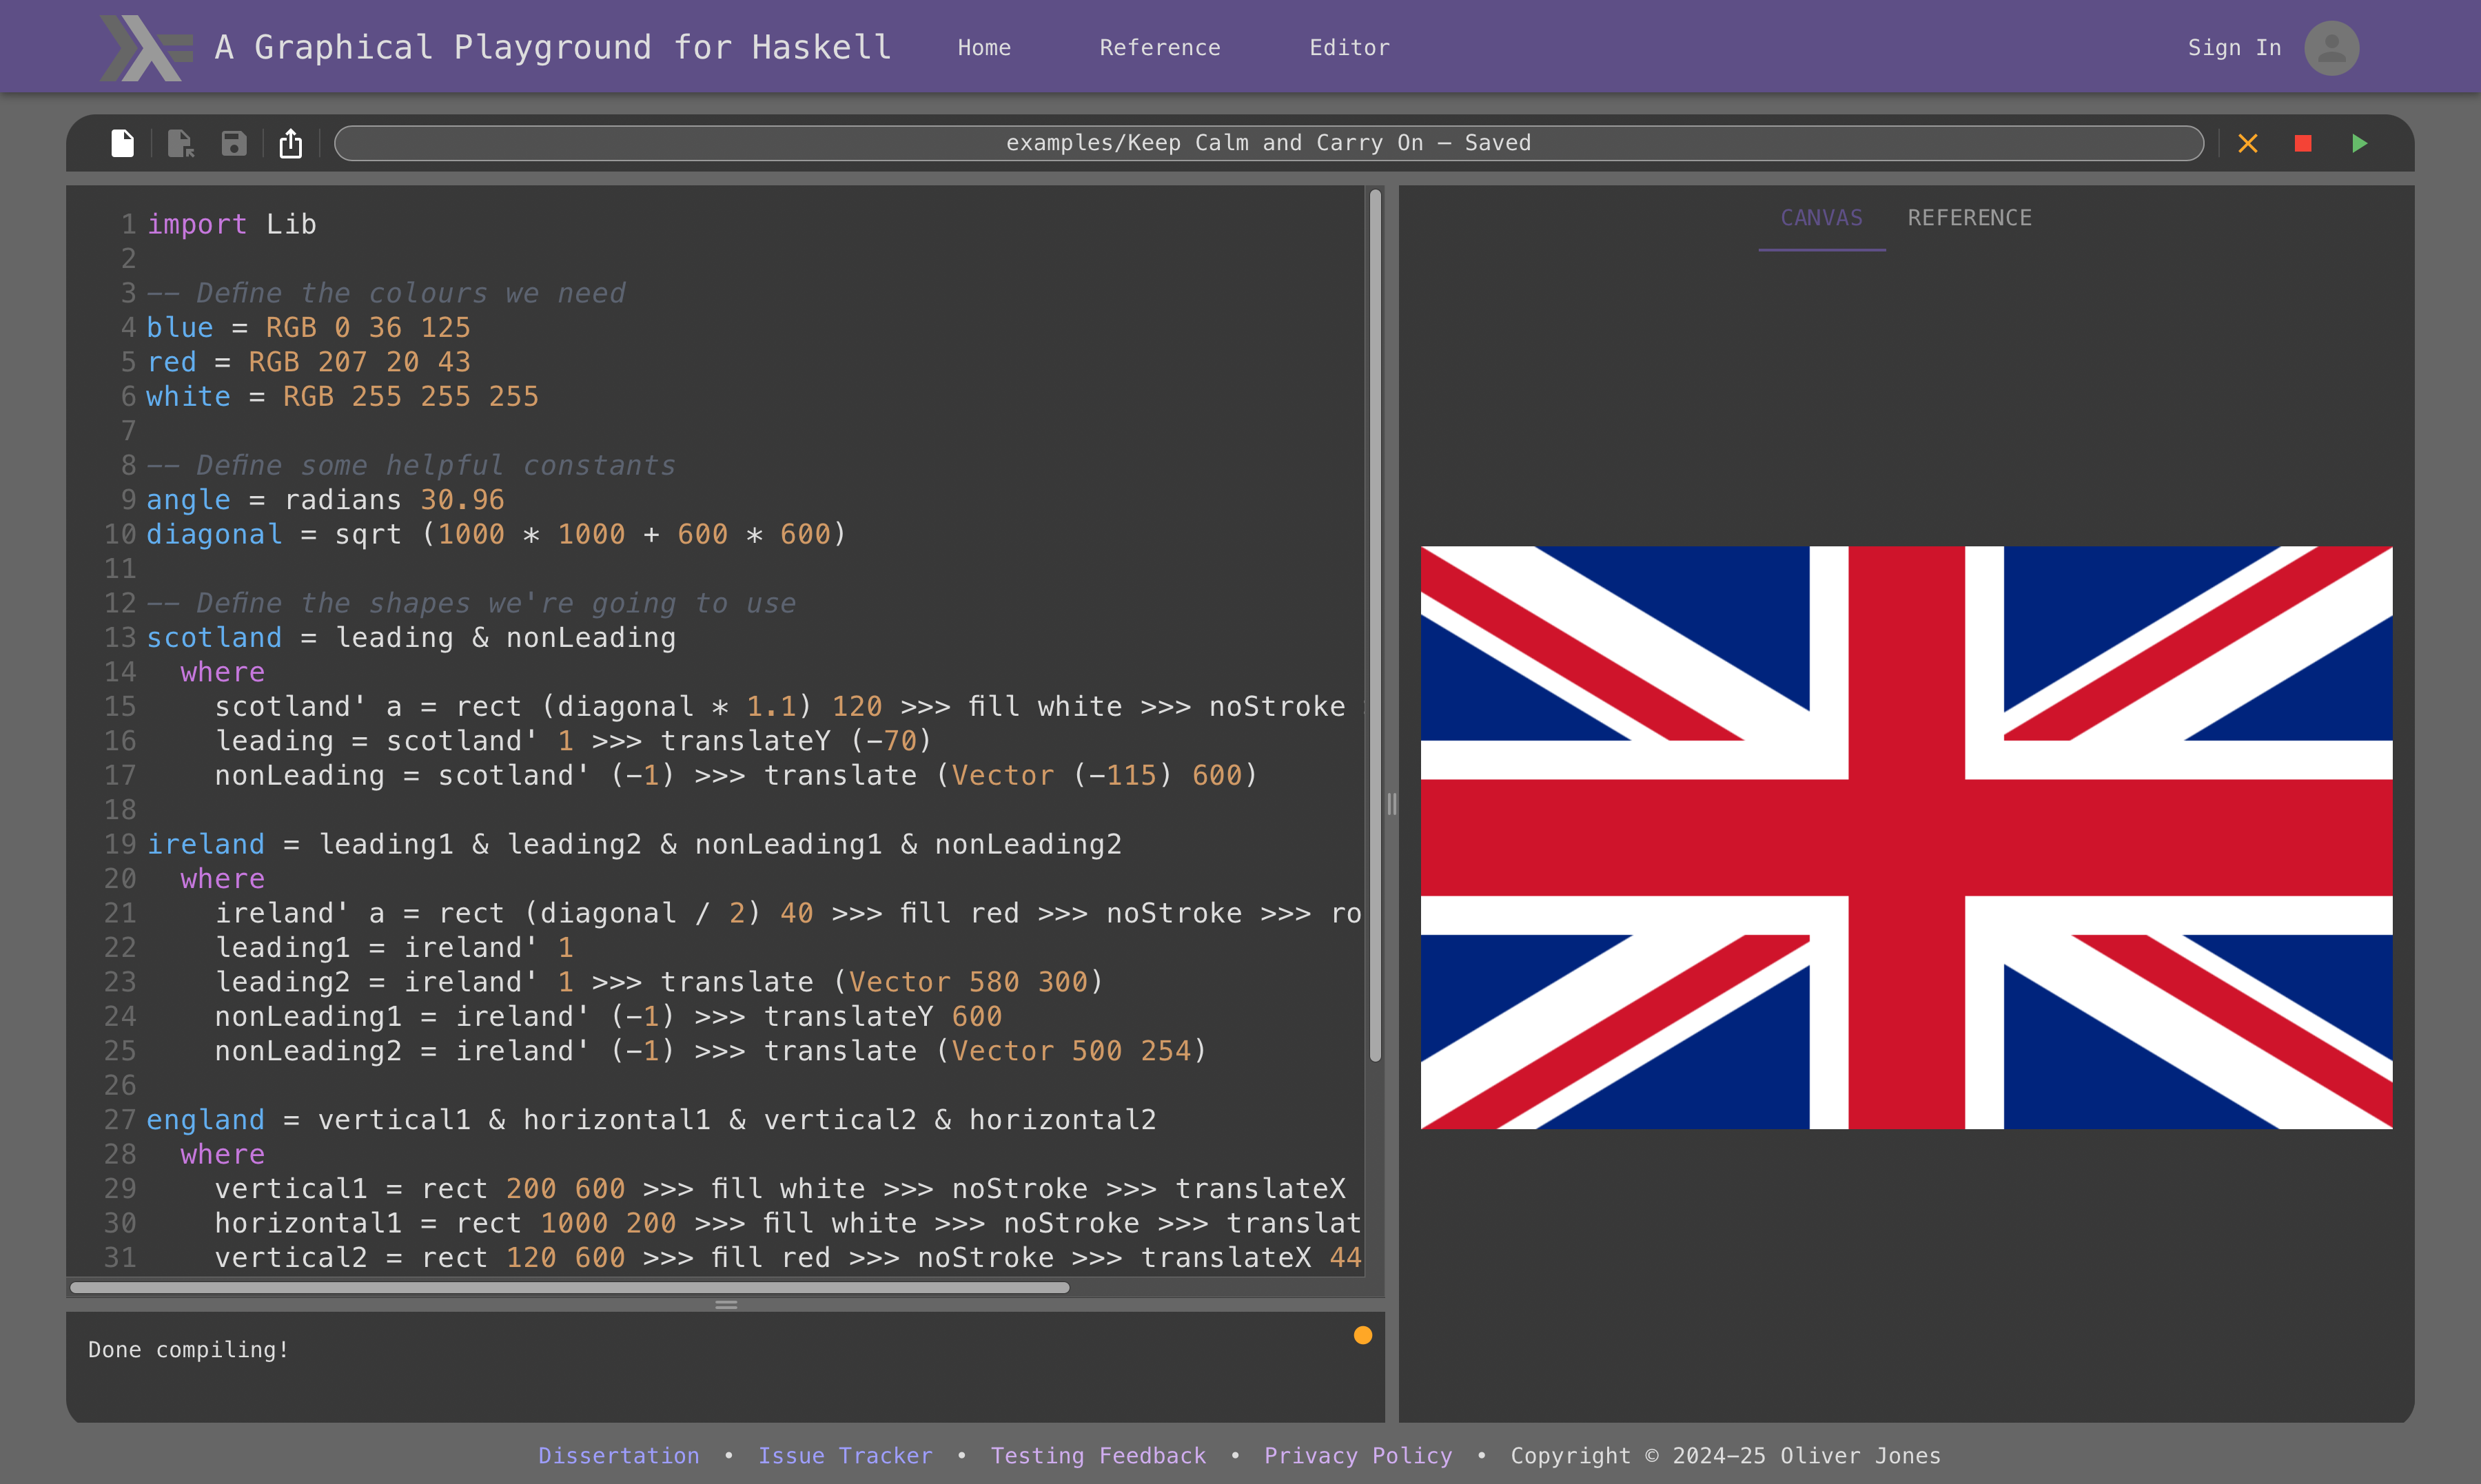
\includegraphics[width=0.9\linewidth]{images/editor.png}
                        \caption{The editor page.
                            The four components outlined can be seen, with the toolbar at the top, the code
                                editor on the left, the graphics display on the right, and the console below
                                the code editor.
                        }
                        \label{fig:editor}
                \end{figure}

                \paragraph{The Code Editor}
                    There is a wide variety of elements built-in to HTML.
                    One of these is the \texttt{<textarea>} element, which can be used to create a
                        multi-line text input field.
                    This element can be used to create a simple code editor, where users can write
                        their Haskell programs.
                    Unfortunately, you cannot change the colour of individual parts of the text in
                        a \texttt{<textarea>} element, so it is not suitable for syntax highlighting.

                    This posed a challenge, as a good code editor should provide syntax
                        highlighting to help users identify different parts of their code.
                    The solution was to layer another element, in this case the \texttt{<pre>}
                        element, behind the \texttt{<textarea>} element, and setting the background and
                        text colours of the \texttt{<textarea>} to \texttt{transparent}.
                    The \texttt{<pre>} element is a block-level element that preserves whitespace
                        and line breaks, making it ideal for displaying code.
                    By setting the CSS \texttt{font-size}, \texttt{line-height} and
                        \texttt{letter-spacing} properties of both the \texttt{<textarea>} and
                        \texttt{<pre>} elements to the same values, the two elements can be made to
                        line up perfectly, creating the illusion that the code is being typed directly
                        into the \texttt{<pre>} element.
                    By adding an event listener to the \texttt{<textarea>} element, the code editor
                        could be made to update the \texttt{<pre>} element with the syntax-highlighted
                        version of the code whenever the user types.
                    A second event listener can be added the \texttt{<textarea>} element to listen
                        for changes in the scroll position, and update the scroll position of the
                        \texttt{<pre>} element accordingly.

                    To achieve syntax highlighting, the code editor uses the \texttt{highlight.js}
                        library, which provides a simple way to add syntax highlighting to code blocks
                        with support for multiple languages, and colour themes.
                    The library produces wraps keywords in \texttt{<span>} elements with a class
                        corresponding to the type of keyword, which can then be styled using CSS.

                    Another useful feature of a code editor is a line number display, which can
                        help users keep track of where they are in their code.
                    To achieve this, each line of the code was split into a separate
                        \texttt{<code>} element.
                    The line number was then displayed using the \texttt{::before} pseudo-element
                        in CSS, which allows developers to insert content before the content of an
                        element.
                    CSS also provides a built-in counter feature, which can be used to
                        automatically number the lines of code.

                \paragraph{The Console}
                    This was the simplest of these components to implement as it is essentially
                        just a text area that displays the output of the user's program.
                    A simple react component which takes a string as a prop and displays it in a
                        text area was all that was needed initially.
                    Later, this component was expanded to include a status indicator, which
                        displays whether the program is currently running, has finished running, or has
                        encountered an error.
                    Originally, this status was indicated by sending a new message to the console,
                        but this proved to be confusing for users.

                \paragraph{The Graphics Display}
                    The original plan for the graphics component was quite simple, just a canvas
                        element, with a function to parse the JSON output of the user's program and
                        draw the graphics on the canvas.
                    However, this proved to be more complex than anticipated.
                    Due to the nature of React, when a component's state updates, the component,
                        and its children are re-rendered.
                    The user's code is stored in the state of the editor component, so when the
                        code changes, the editor component is re-rendered, triggering all of its
                        children to re-render as well.
                    This posed an issue for the graphics component, as every re-render would, at
                        best, cause a small flicker as the rendered image is re-rendered, and at worst,
                        cause an animation to restart.

                    Fortunately, React provides a solution to the problem of re-rendering child
                        components every time the parent component re-renders.
                    By using the \texttt{React.memo} function, the graphics component can be
                        memoised, meaning that it will only re-render when its props change.
                    This solves the issue of the graphics component re-rendering every time the
                        editor component re-renders.

                    With this solution, it was straightforward to wait for the user's program to
                        finish running, and then parse the JSON output and draw the graphics on the
                        canvas.
                    However, this meant that the user had to wait for the program to finish running
                        before they could see the graphics.
                    By implementing an intermediate controller component, the graphics could be
                        drawn as the program runs, allowing the user to see the graphics being drawn in
                        real-time.
                    This intermediate component is also memoised, so it only re-renders as more
                        data is received from the server.
                    It is then responsible for parsing the JSON data, and passing it to the
                        graphics component to be drawn on the canvas at the correct time, accounting
                        for the frame rate of the graphics.

                    To summarise, the graphics display component has two parts: the controller
                        component, which receives the output of the user's program from the server and
                        passes it to the graphics component, and the graphics component, which draws
                        the graphics on the canvas.
                    The controller ensures that animations are drawn at the correct frame rate, and
                        that the graphics are drawn in real-time as the program runs.

                \paragraph{The Toolbar}
                    The toolbar component is a simple row of buttons that allow users to control
                        their programs.
                    In the centre of the toolbar, the name of the program is displayed, along with
                        the name of the user who wrote it.
                    To the left of this, there are four buttons: new, save, open and share.
                    As the names suggest, these buttons allow users to create a new program, which
                        replaces the content of the code editor with some boilerplate code, save their
                        current program, open a saved program, and share their program with others.
                    Saving and opening programs are only available to users who are logged in,
                        while sharing is available to all users.
                    Sharing gives the user the option of copying their program to the clipboard,
                        generating and copying a URL which links directly to the program, copying the
                        image output of the program to the clipboard, or downloading the image output
                        of the program.
                    To the right of the program name are three buttons: clear, run and stop.
                    The clear button clears the console and graphics display, the run button runs
                        the user's program, and the stop button stops the program if it is currently
                        running.

        \subsection{Making the Components Resizeable}
            Making the components resizeable was relatively straightforward.
            By creating a component to handle a split view, and using this component twice
                to create a three-way split view, the editor page was made resizeable.
            The split view component takes two child components, and allows the user to
                drag the border between them to resize them.
            By laying out the editor page thus: \begin{lstlisting}[caption={A simplified version of the editor page layout.},
                label={lst:editorLayout}]
<SplitView>
    <SplitView vertical>
        <CodeEditor />
        <Console />
    </SplitView>
    <GraphicsController />
</SplitView>\end{lstlisting} the editor page was
                made resizeable, with the code editor and console components contained in a
                column on the left, with a resizeable border between them, and the graphics
                controller component on the right, with a resizeable border between it and the
                column on the left.

        \subsection{Making a Reference Page}
            The reference page was considerably simpler to implement than the editor page.
            It is simply a long page of text, with a table of contents at the top, which
                links to the various sections of the page.
            The page is divided into sections, with alternating coloured backgrounds to
                make it easier to read, with each section detailing a different aspect of the
                graphics library.
            The sections are:
            \begin{itemize}
                \item ``Haskell'', which brief explanation of Haskell's \texttt{Prelude} module, with a link to its
                      full documentation, and an explanation of Haskell's type signature syntax.
                \item ``Canvas'', which explains the concept of the canvas, and how to create it.
                \item ``Images and Animations'', which explains how to draw images and animations on the canvas and
                      modify the frame rate and background colour.
                \item ``Vectors'', which explains how to create and manipulate vectors.
                \item ``Shapes'', which explains how to create the various shapes available in the graphics library,
                      with pictures of each shape.
                \item ``Transformations'', which explains how to manipulate these shapes, with pictures of each
                      transformation.
                \item ``Colors'', which explains how to create colours using the various colour spaces available in
                      the graphics library.
                \item ``Other'', which explains how to use the other functions available in the graphics library.
            \end{itemize}

            Throughout the page are a series of examples, which demonstrate how to use the
                various functions available in the graphics library.
            These examples are written in both inline and block code, which are styled
                accordingly to make them clear.

            The ``Color'' section also includes a list of all the named colours available
                in the graphics library, shown in Figure~\ref{fig:colours}.
            Each colour is displayed as its name, highlighted in that colour.
            Hovering over these names displays a tooltip with the hexadecimal, RGB and HSL
                values of the colour.
            The list can be sorted either by colour, a combination of hue, then saturation,
                then lightness, or alphabetically by name, to accommodate users who are
                colour-blind.

            \begin{figure}[H]
                \centering
                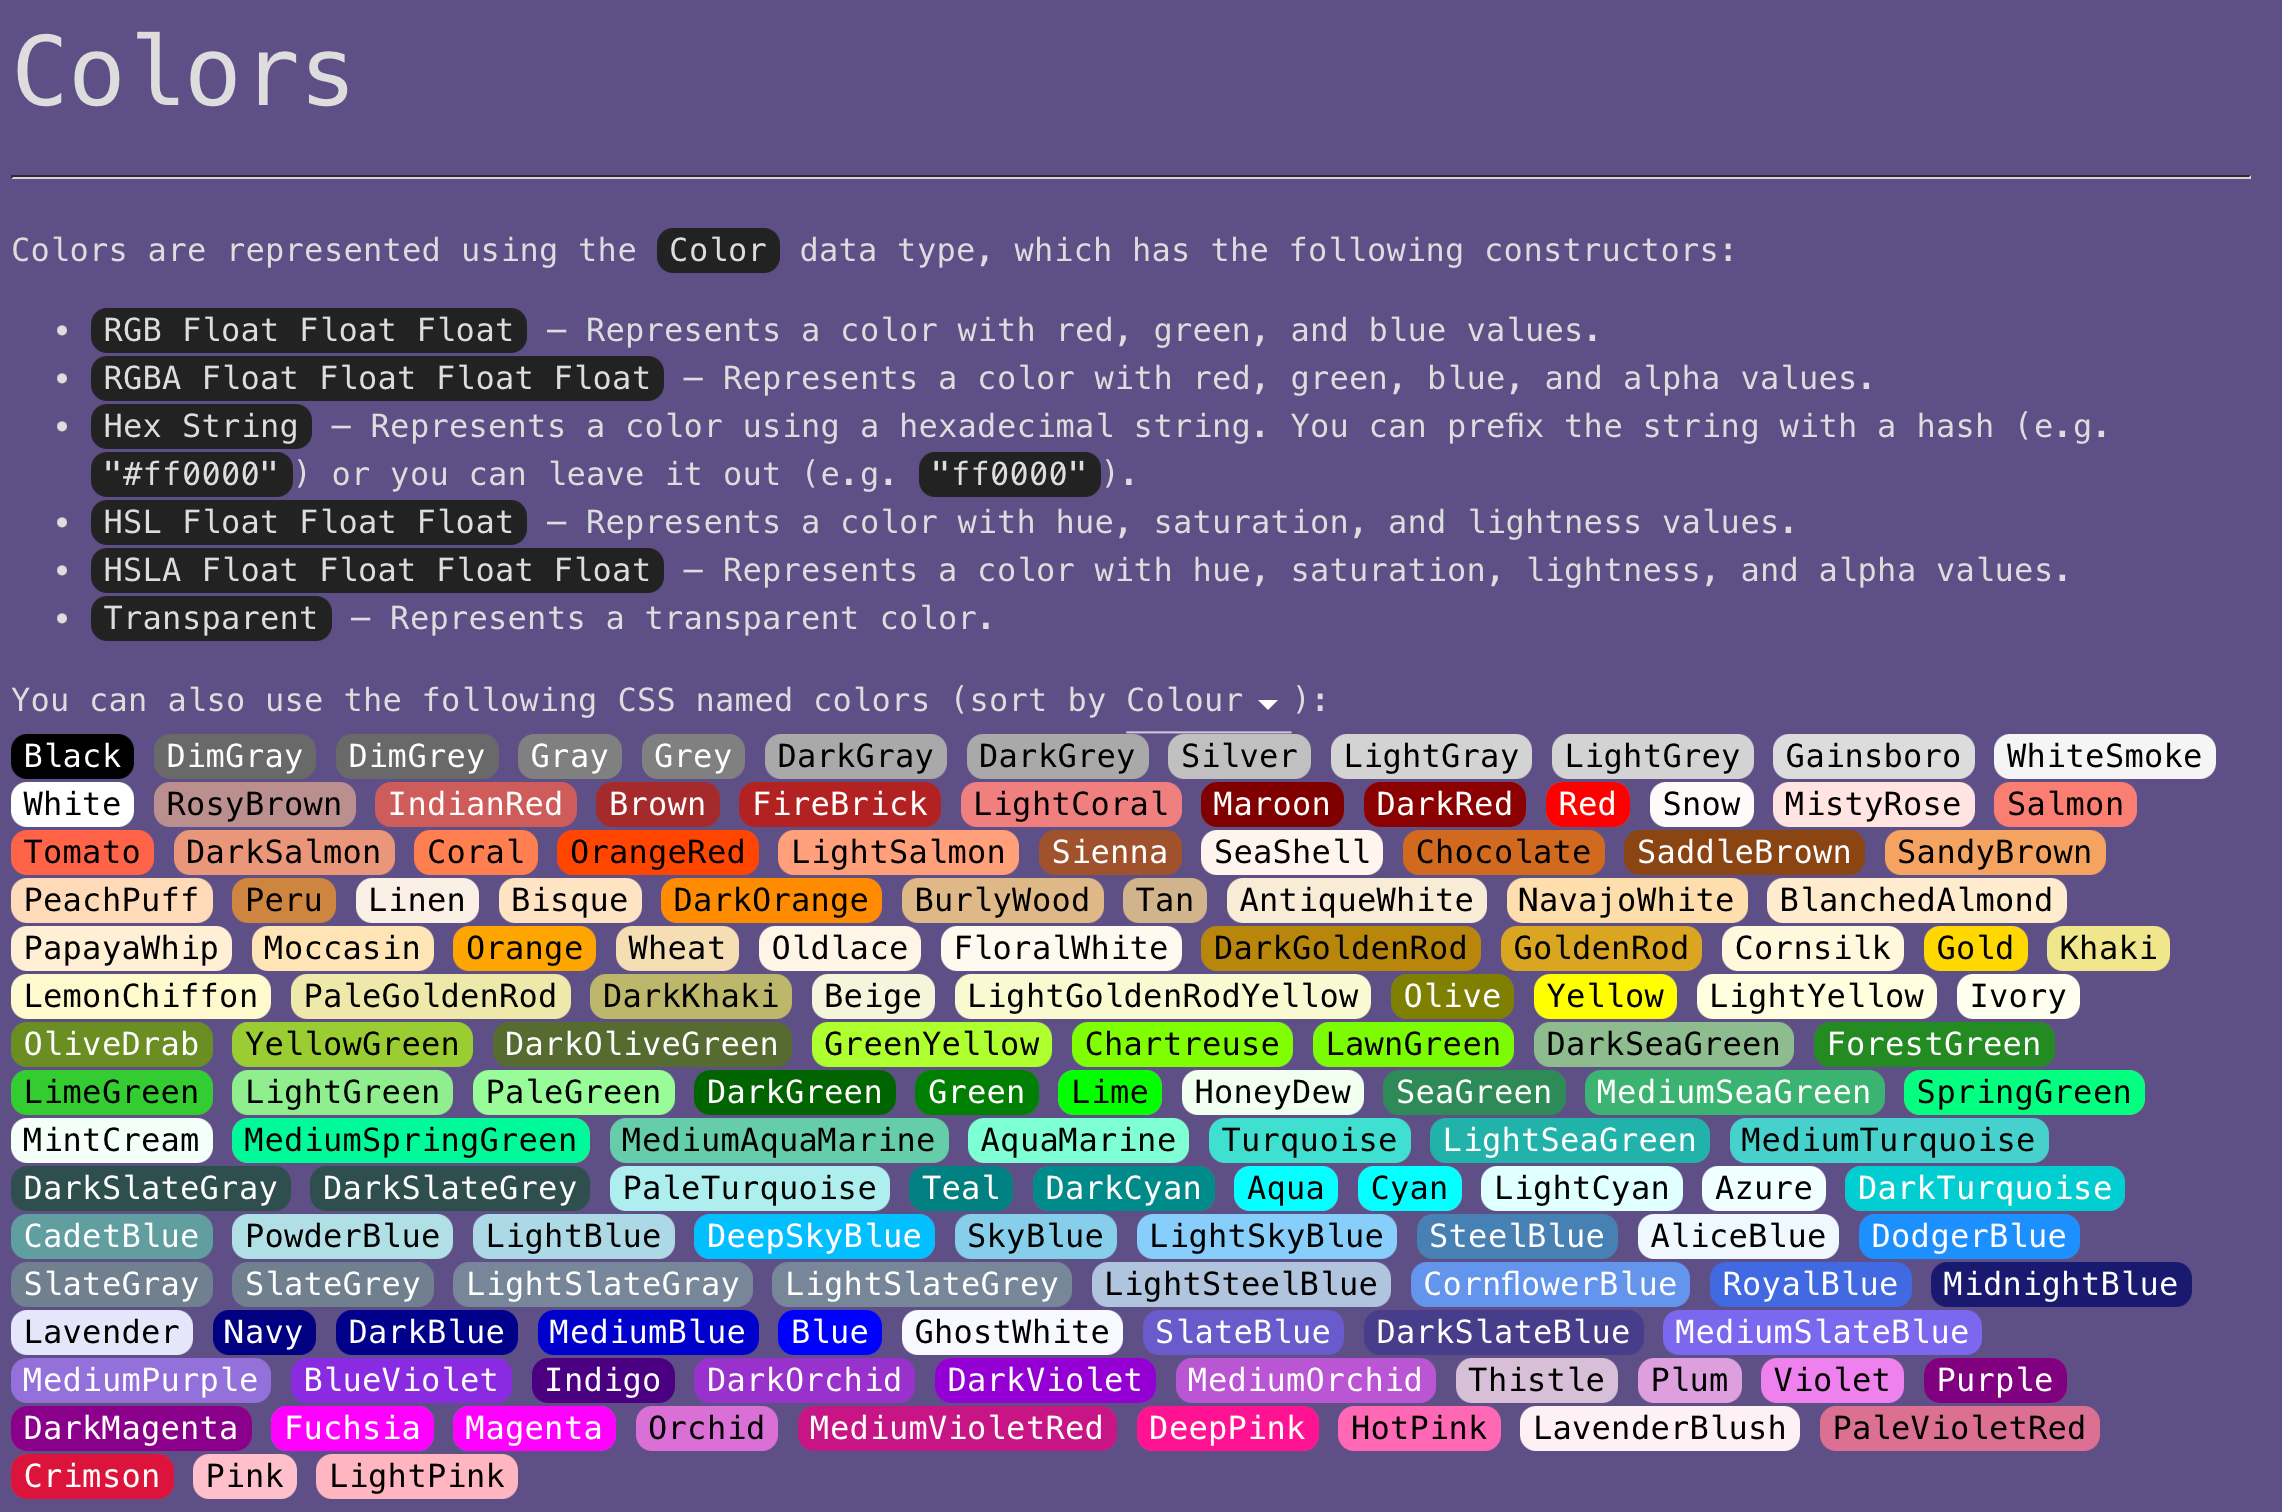
\includegraphics[width=0.45\linewidth]{images/colours.png}
                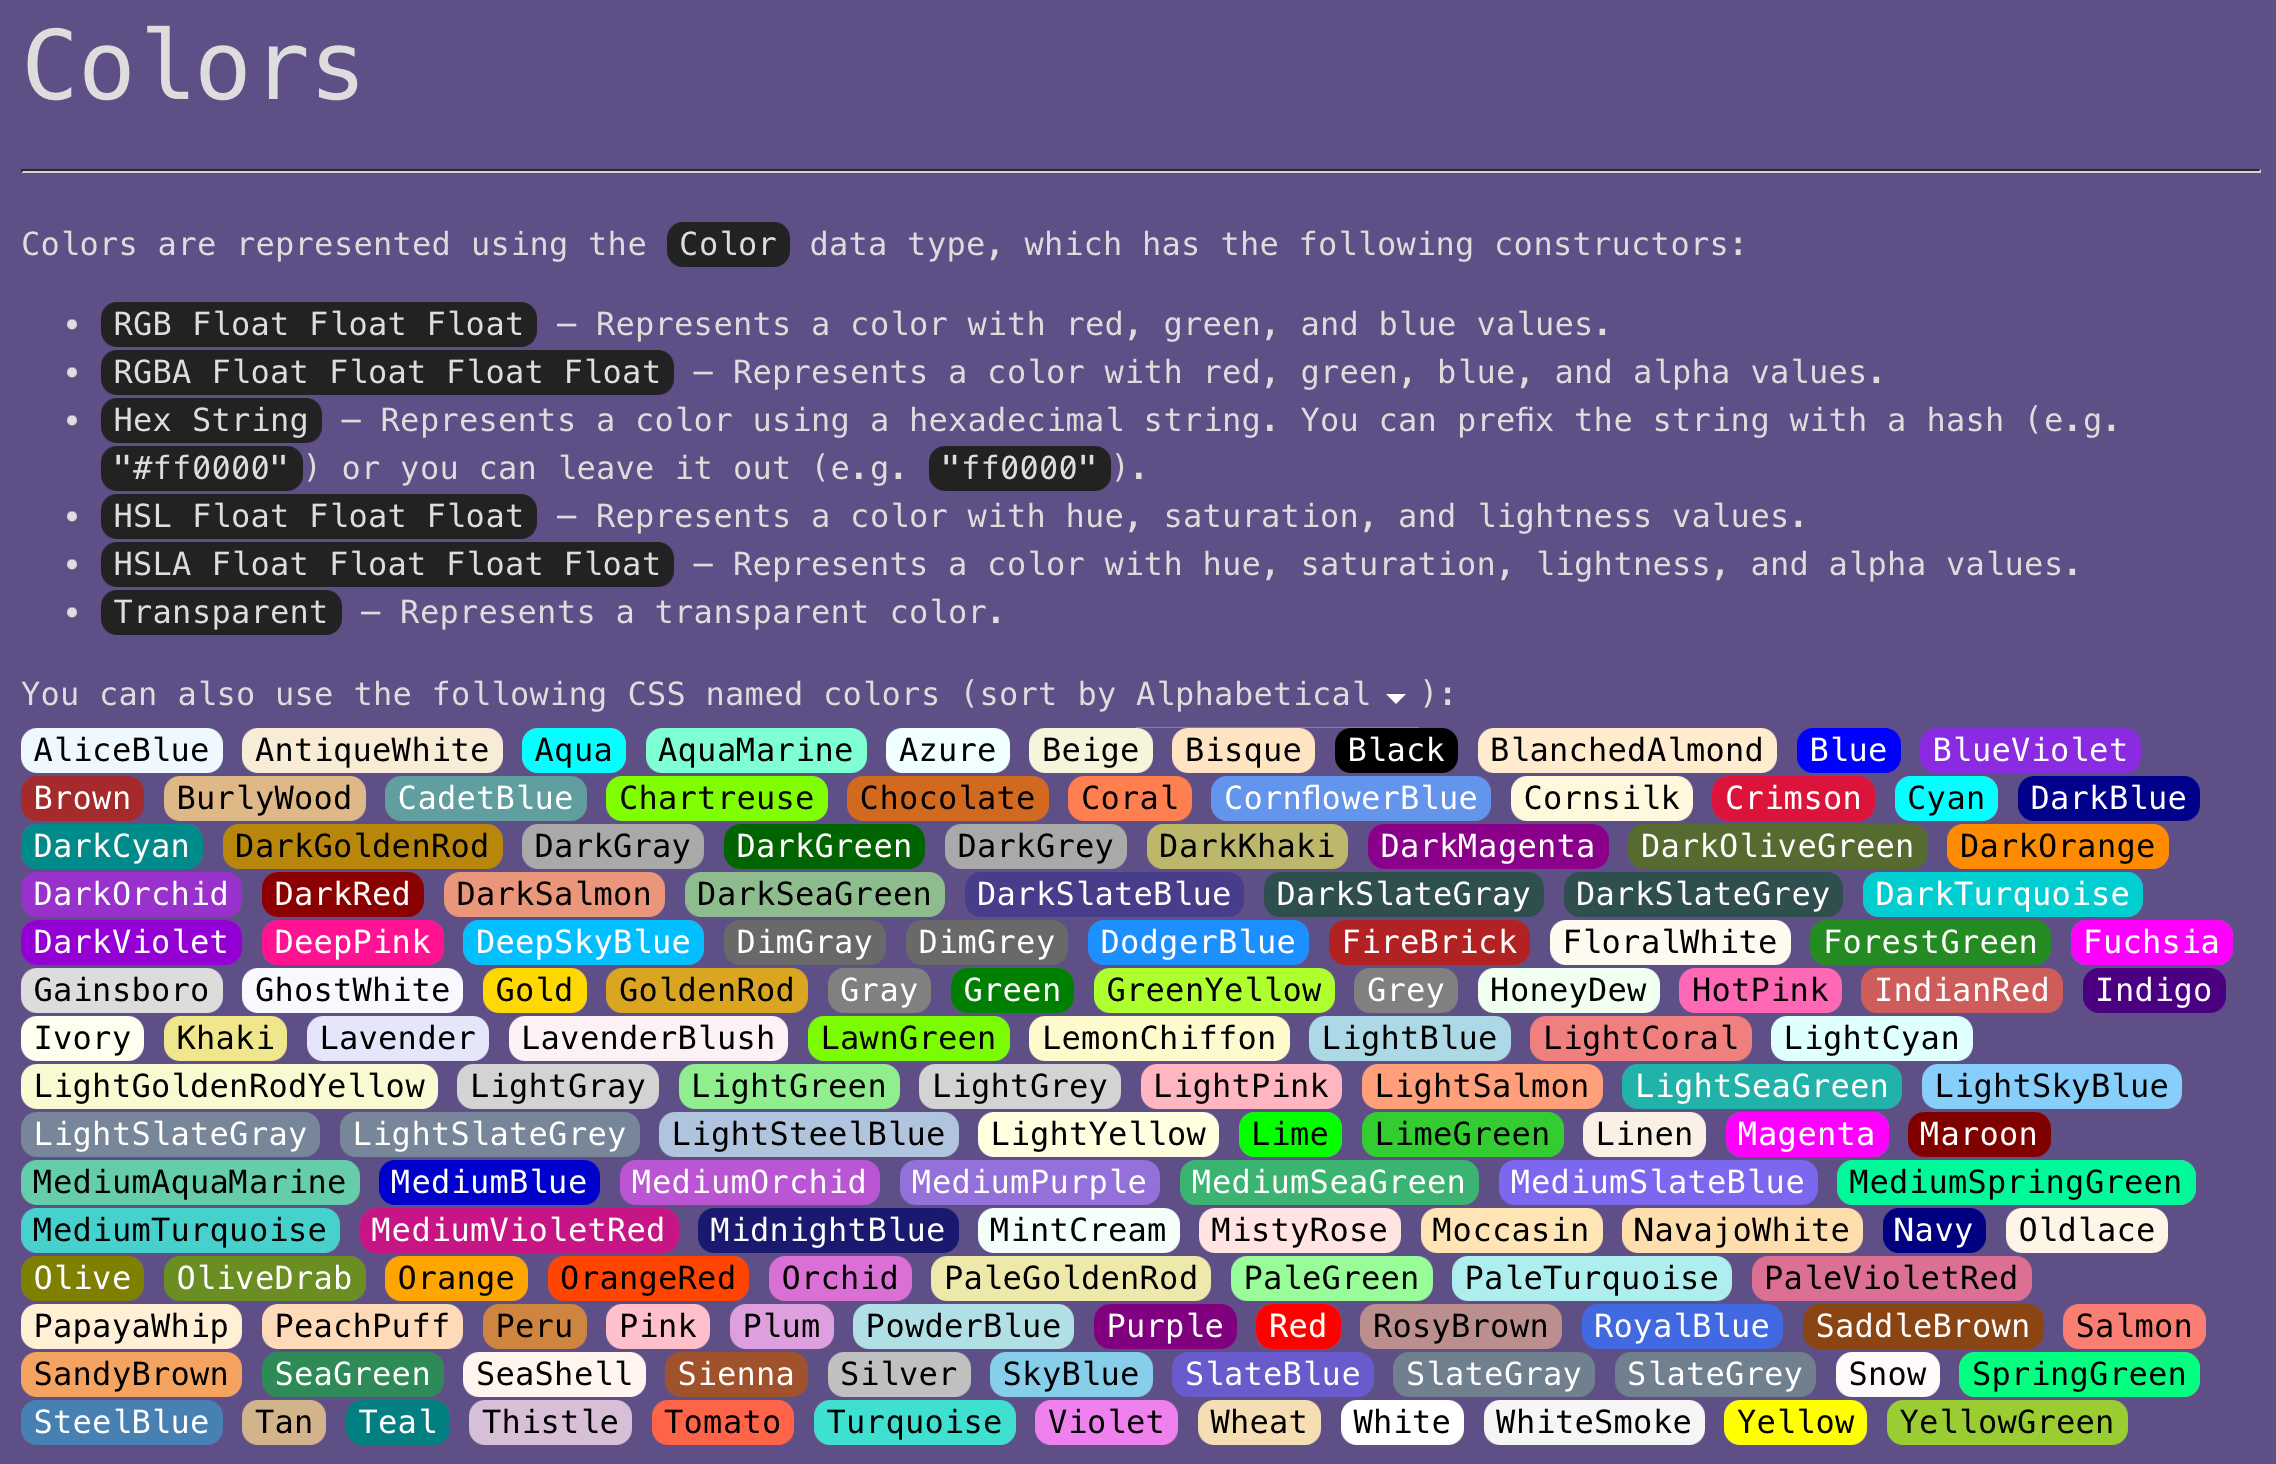
\includegraphics[width=0.45\linewidth]{images/coloursAlphabetical.png}
                    \caption{The ``Colors'' section of the reference page.
                        On the left, the colours are sorted by hue, saturation, and lightness.
                        On the right, the colours are sorted alphabetically.
                    }
                    \label{fig:colours}
            \end{figure}

            In response to feedback from multiple users, the reference page can also be
                accessed directly from the editor page, by clicking the ``Reference'' above the
                canvas.
            This replaces the graphics display with the reference page, allowing users to
                quickly look up information about the graphics library without leaving the
                editor page.

        \subsection{Creating a User Account System}
            User accounts are nothing new to the internet.
            They are used for storing user data, and to provide a more personalised
                experience for the user.
            For this website, user accounts are used to store the user's saved programs.

            Next.js provides built-in support for middleware, which can be used to direct
                users to the correct page based on their authentication status.
            Users who are not logged in, who try to access the \texttt{/account} page, are
                redirected to the login page.
            Users who are logged in, who try to access the login page, are redirected to
                the account page.
            This ensures that users are always directed to the correct page, based on their
                authentication status.

            The user account system is relatively simple.
            Users can create an account by providing an email address and password.
            The password is hashed using the \texttt{bcrypt} library, and the email address
                is stored in plain text.
            When a user logs in, the server checks the email address and password against
                the database, and if they match, the user is logged in.
            A unique identifier is generated for the user, and stored in a cookie, which is
                sent to the client.
            This cookie is used to authenticate the user on subsequent requests, so they do
                not need to log in every time they try to access a protected endpoint.

            The user account system also allows users to save their programs.
            When a user saves a program, it is stored in the database, along with the
                user's unique identifier.
            When a user logs in, the server retrieves all the programs associated with that
                user's unique identifier, and displays them on the account page.

        \subsection{Landing on the Homepage}
            The homepage is the first page users see when they visit the website.
            It is designed to be engaging and informative, showcasing the capabilities of
                the graphics library, and encouraging users to try it out.

            \begin{figure}[H]
                \centering
                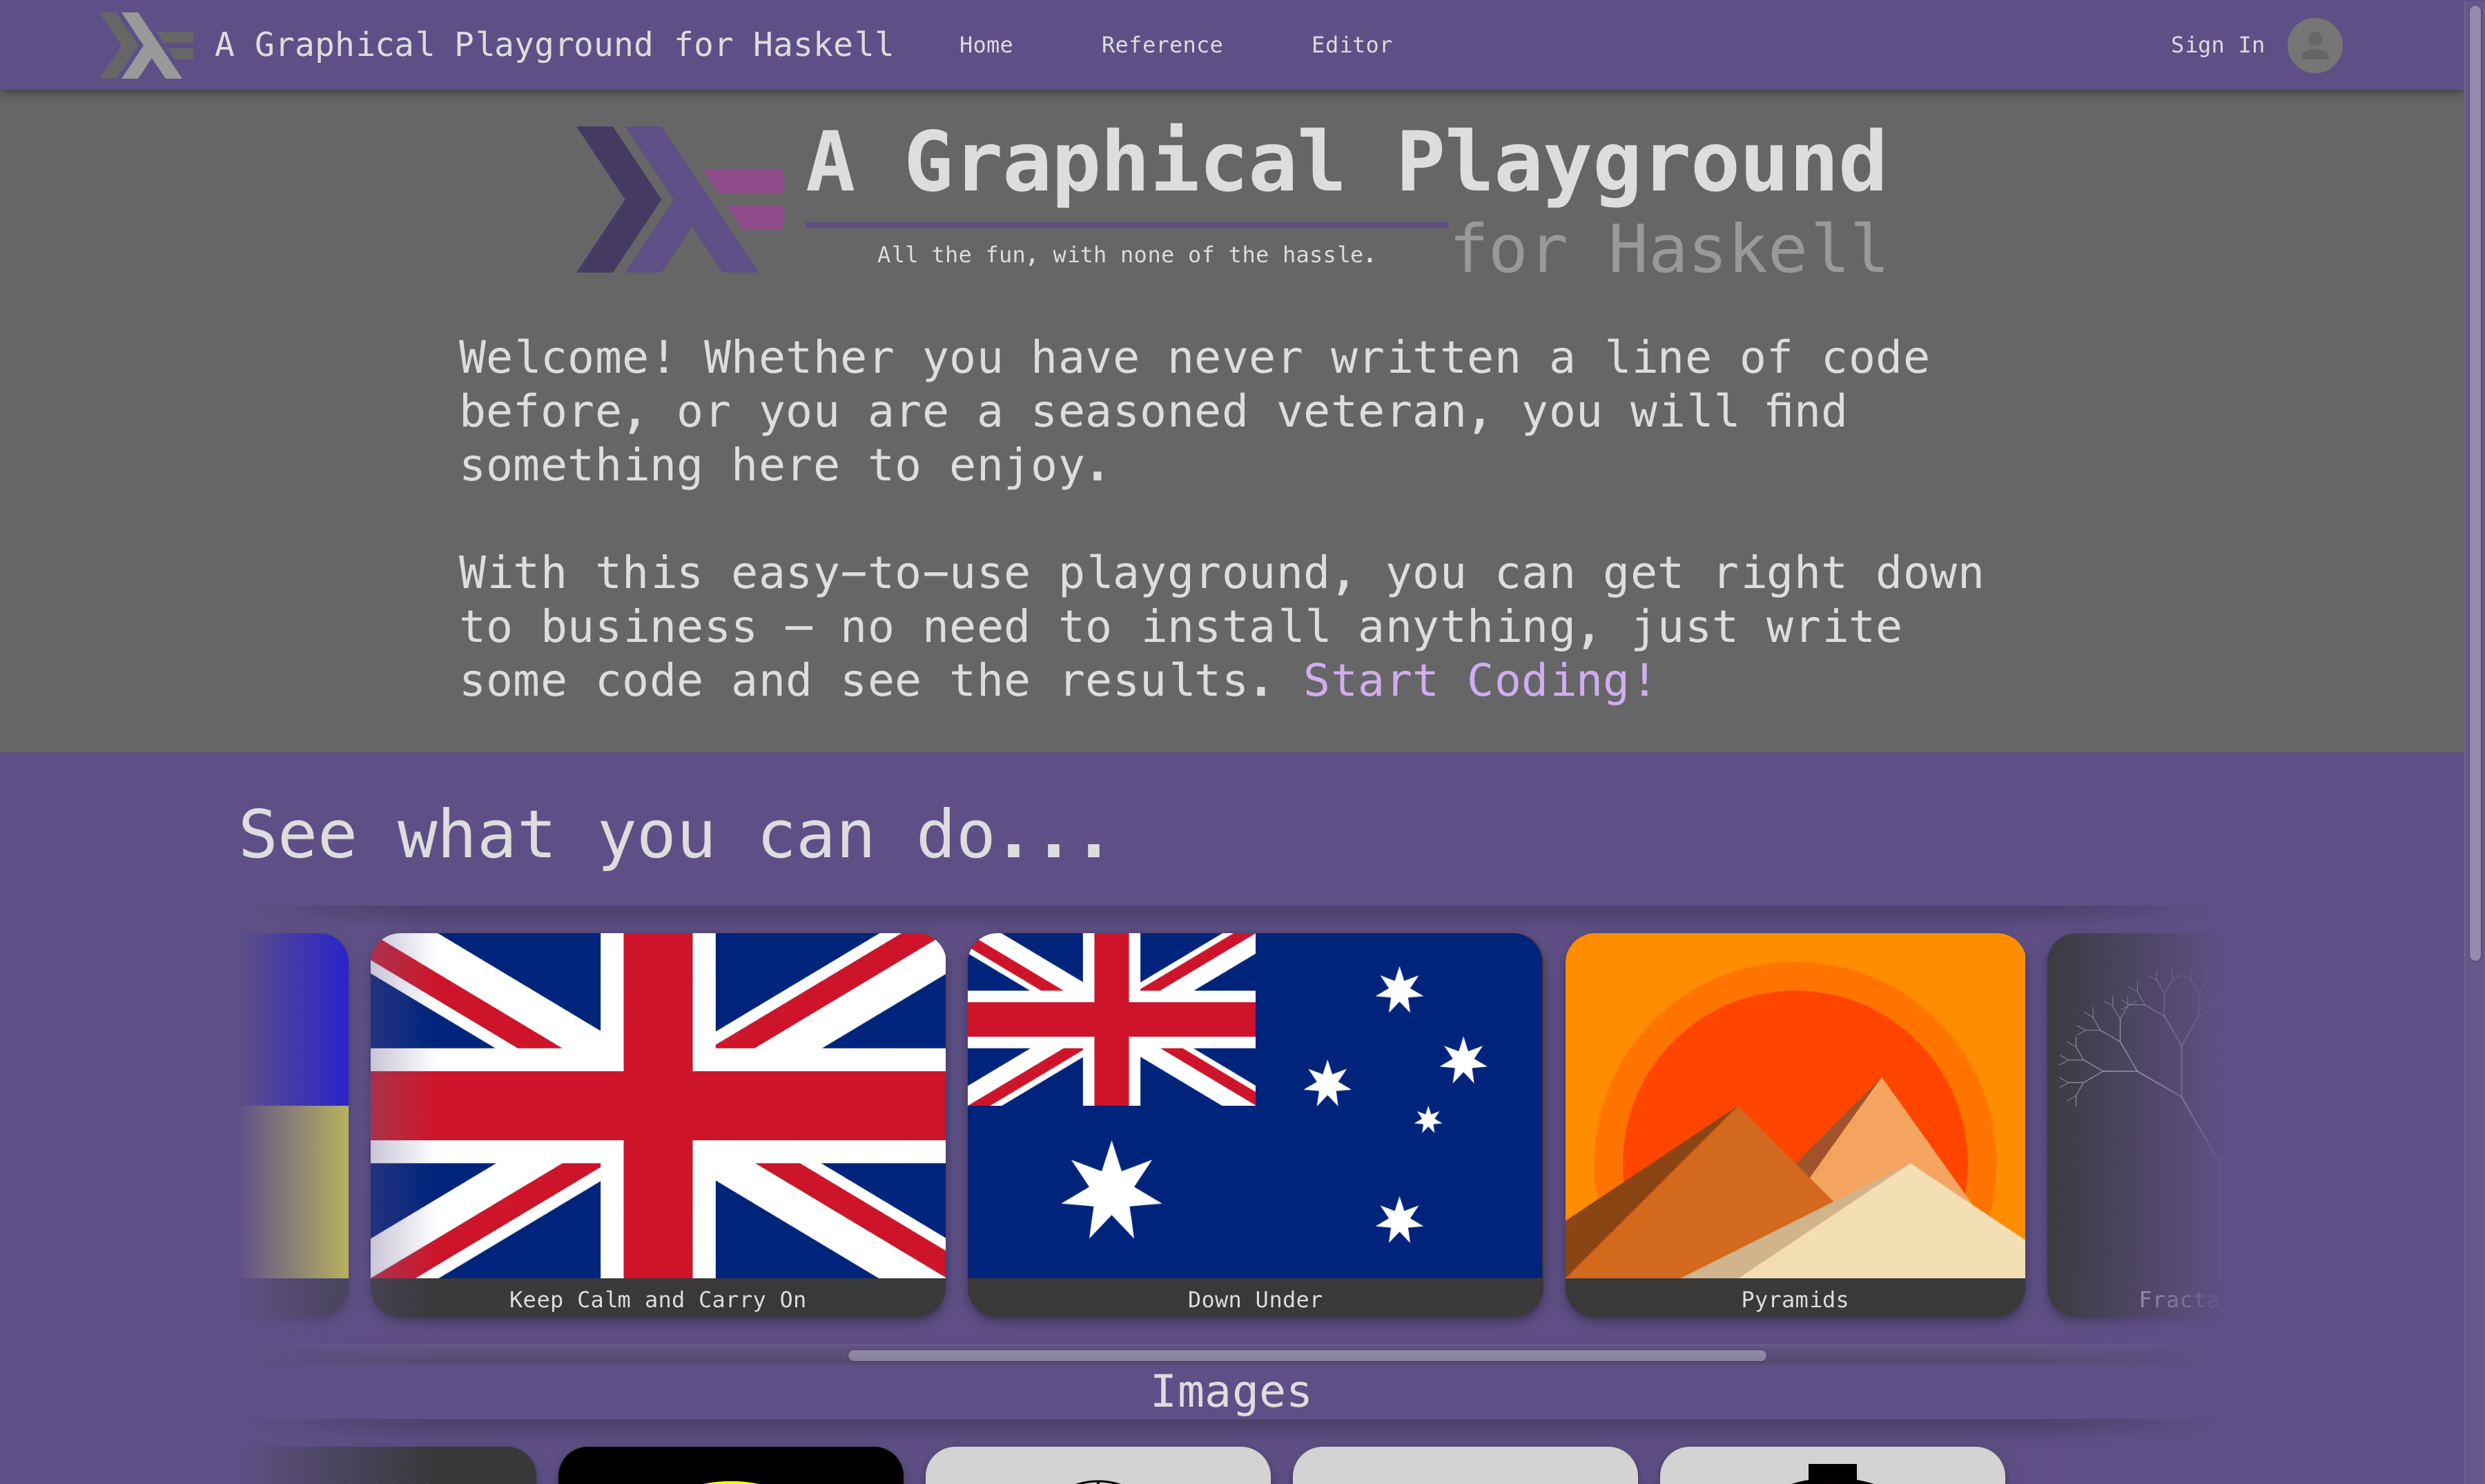
\includegraphics[width=0.9\linewidth]{images/homepage.png}
                    \caption{The homepage.}
                    \label{fig:homepage}
            \end{figure}

            The top of the homepage features a large banner, indicating the name of the
                website, and a very brief description of its purpose.
            Below is a brief welcome message to the user, encouraging them to try out the
                graphics library.
            Below this is a series of examples, showcasing the capabilities of the graphics
                library — both static images and animations.
            Finally, at the bottom of the page is a help section, directing users to the
                reference page for more information about the graphics library, and to the
                issue tracker if they encounter any problems.

        \subsection{Quality-of-Life and Legal Requirements}
            There are a few quality-of-life features that were added to the website to make
                it more user-friendly.
            These include:
            \begin{itemize}
                \item A notification banner which displays at the bottom corner of the screen
                      whenever a user carries out certain actions such as saving a program, copying
                      their program or URL via the share, etc.
                      This also shows a notification informing the user that the website uses
                          cookies, as is legally required by GDPR regulations.
                      The banner automatically fades after a few seconds, but does not disappear
                          entirely until the user dismisses it.
                \item The footer includes links to this dissertation, the GitHub issue tracker,
                      the user testing and feedback form, and the privacy policy.
                      It also includes a copyright notice.
                \item A saved state indicator appears in the menu bar, informing a user of whether
                      they have an open program, and if it is saved.
                      Hovering over this indicator displays a tooltip with the name of the program.
                \item Confirmation menus appear when a user tries to open a program while they
                      have an unsaved program open, preventing them from losing their work.
                      The same is true when a user tries to delete one of their saved programs.
            \end{itemize}

\end{document}
